\documentclass[aspectratio=169,final]{beamer}
\setbeamersize{text margin left=5pt,text margin right=5pt}
\setbeamertemplate{navigation symbols}{}



\usepackage{booktabs}
\usepackage{multirow}
\usepackage{tikz}
\usetikzlibrary{arrows.meta}
\usetikzlibrary{calc}
%\usetikzlibrary{arrows,shapes}
\usetikzlibrary{fit,bayesnet}


\usepackage{amsmath}
\newcommand{\expect}{\mathds{E}} %{{\rm I\kern-.3em E}}
\newcommand{\probability}{\mathds{P}} %{{\rm I\kern-.3em P}}
\newcommand{\indicator}{\mathds{1}} %{{\rm I\kern-.3em P}}
\DeclareMathOperator*{\argmax}{arg\,max} % thin space, limits underneath in displays
\DeclareMathOperator*{\argmin}{arg\,min} % thin space, limits underneath in displays
\newcommand{\code}[1]{{\texttt{#1}}}
\newcommand{\scode}[1]{{\texttt{#1}}}
\newcommand{\codechar}[1]{{\texttt{"#1"}}}

\usepackage{xcolor}
\definecolor{pop1}{HTML}{1F78b4}
\definecolor{pop2}{HTML}{164C13}
\definecolor{pop3}{HTML}{d95F02}
\definecolor{orange}{HTML}{d95F02}
\definecolor{teal}{HTML}{1b9e77}
\newcommand{\pop}[1]{\textcolor{pop1}{#1}}
\newcommand{\popp}[1]{\textcolor{pop2}{#1}}
\newcommand{\tree}[1]{\textcolor{pop3}{#1}}
\newcommand{\orange}[1]{\textcolor{orange}{#1}}
\newcommand{\teal}[1]{\textcolor{teal}{#1}}
\newcommand\Wider[2][3em]{%
\makebox[\linewidth][c]{%
  \begin{minipage}{\dimexpr\textwidth+#1\relax}
  \raggedright#2
  \end{minipage}%
  }%
}

\begin{document}

\begin{frame}{\centering  Library Learning for Neurally-Guided Bayesian Program Induction\\
    \centering\small  Kevin Ellis$^1$, Lucas Morales$^1$, Mathias Sabl\'e-Meyer$^2$,\\ Armando Solar-Lezama$^1$, Joshua B. Tenenbaum$^1$\\
  \small   $^1$: MIT. $^2$: ENS Paris-Saclay.}

  \begin{minipage}[c]{0.3\textwidth}
\centering        \underline{List processing:}\vspace{-0.3cm}\begin{align*}
    \code{[5 2 9]}&\to\code{[9 2 5]}\\
    \code{[1 1 2 2]}&\to\code{[2 2 1 1]}\\
    \code{[1 2 3 2]}&\to\code{[2 3 2 1]}\\
    %% &\\
    %% \code{[9 8 2]}&\to\code{[8 2]}\\
    %% \code{[0 3 0 0]}&\to\code{[3 0 0]}\\
    %% \code{[2 1]}&\to\code{[1]}
    \end{align*}
  \end{minipage} $\quad$
  \begin{minipage}[c]{0.3\textwidth}
\centering            \underline{Text editing:}\vspace{-0.3cm}\begin{align*}
      \text{P Kohli}&\to\text{Dr. Kohli}\\
      \text{Sumit Gulwani}&\to\text{Dr. Gulwani}\\
      \text{Danny Tarlow}&\to\text{Dr. Tarlow}\\
    %%   &\\
    %% \text{+106 769-438}&\to\text{106.769.438}\\
    %% \text{+83 973-831}&\to\text{83.973.831}\\
    %% \text{+882 101-723}&\to\text{882.101.723}    
      \end{align*}    
    \end{minipage} $\quad$
  \begin{minipage}[c]{0.3\textwidth}
\centering            \underline{Symbolic regression:}\\\begin{tabular}{cc}
      
\includegraphics[width = 3em]{figures/functions/92.png}&
      
\includegraphics[width = 3em]{figures/functions/146}\\
      \begin{tabular}{c}
                  $ax^3 + bx^2 +$\\$ cx + d$
        \end{tabular}
      &    $a/(x - b)$\\
      ~\\
      %% 
\includegraphics[width = 3em]{figures/functions/112.png}&
      %%   
\includegraphics[width = 3em]{figures/functions/92.png}
%%         \\
%%         \begin{tabular}{c}
%% $          ax^4 + bx^3 + $\\$cx^2 + dx + e$
%%           \end{tabular}

%%         &\begin{tabular}{c}
%%            $ax^3 + bx^2 +$\\$ cx + d$
%%            \end{tabular}

    \end{tabular}
    
  \end{minipage}

  \vspace{1cm}
  Explore/Compress/Compile (EC$^2$) learns to solve programming tasks like these by growing a library of code and training a neural net to search for programs written using the library

  \end{frame}

\begin{frame}{Library Learning}
\centering
  \renewcommand\code\texttt
  \renewcommand\codechar[1]{\texttt{"#1"}}
  \newcommand{\helpSize}{0.25cm}
\begin{tabular}{cc}
    \toprule
Tasks and     \pop{Programs} & DSL\\
    \midrule
      \begin{tabular}{cc}
        \begin{tabular}{c}
          \code{[7\, 2\, 3]}$\to$\code{[7\, 3]}         \\
          \code{[1\, 2\, 3\, 4]}$\to$\code{[3\, 4]} \\
          \code{[4\, 3\, 2\, 1]}$\to$\code{[4\, 3]} \\
          \pop{\code{$f(\ell) = $}\code{($f_1$ $\ell$ ($\lambda$ (x)}}\\
          \hspace{1.15cm}\pop{\code{(> x 2)))}}       \\
          \\
          \\
          \code{[2\, 7\, 8\, 1]}$\to $\code{8}               \\
          \hspace{0.15cm}\code{[3\, 19\, 14]}$\to $\code{19}                \\
          \pop{\code{$f(\ell) = $}\code{($f_2$ $\ell$)}}
        \end{tabular}
        &
        \hspace{-0.3cm}\begin{tabular}{c}
          \code{[7\, 3]}$\to $\code{False}                              \\
          \hspace{0.3cm}\code{[3]}$\to $\code{False}                    \\
          \hspace{-0.3cm}\code{[9\, 0\, 0]}$\to $\code{True\phantom{e}} \\
          \hspace{0.3cm}\code{[0]}$\to $\code{True\phantom{e}}                        \\
          \hspace{-0.3cm}\code{[0\, 7\, 3]}$\to $\code{True\phantom{e}}                \\
          \pop{\code{$f(\ell) = $}\code{($f_3$ $\ell$ 0)}}
        \end{tabular}
      \end{tabular}
    &
    \begin{tabular}{l}
      \popp{$f_0(\ell,$\code{r}$) \,=\, $\code{(foldr r $\ell$ cons)}}\\
      \hspace{\helpSize}($f_0$: \emph{Append lists }\code{r}\emph{ and  $\ell$})\\
      \popp{$f_1(\ell,$\code{p}$) \,=\, $\code{(foldr $\ell$ nil ($\lambda$ (x a)}}\\
      \hspace{0.5cm}\popp{\code{(if (p x) (cons x a) a)))}}\\
      \hspace{\helpSize}($f_1$: \emph{Higher-order filter function})\\
      %(lambda (fold $0 0 (lambda (lambda (if (gt? $0 $1) $0 $1)))))
      \popp{$f_2(\ell) \,=\, $\code{(foldr $\ell$ 0 ($\lambda$ (x a)}}\\
      \popp{\phantom{$f_2(\ell) \,=\, $}\code{(if (> a x) a x)))}}\\
      \hspace{\helpSize}($f_2$: \emph{Maximum element in list $\ell$})\\
      \popp{$f_3(\ell,$\code{k}$) \,=\, $\code{(foldr $\ell$ (is-nil $\ell$)}}\\
      \phantom{$f_1(\ell,$}
      \popp{\code{($\lambda$ (x a) (if a a (= k x))))}}\\
      \hspace{\helpSize}($f_2$: \emph{Whether $\ell$ contains }\code{k})\\
    \end{tabular}
  \\\bottomrule
  \end{tabular}
  \begin{itemize}
  \item Learned DSL primitives can call each other
    \item Rediscovers higher-order functions like \code{filter}
    \end{itemize}
\end{frame}

\begin{frame}{Explore/Compress/Compile as {\color{red}Amortized} Bayesian Inference}
  
\newcommand{\NeuralNetwork}[1]{    \begin{tikzpicture}[x=2.5cm,y=1.25cm,transform canvas={scale=#1,shift={+(-1,2.5)}}]
      \tikzstyle{neuron}=[circle,fill=blue!50,minimum size=20pt]
      \fill[fill=white] (-0.25,-0.5) rectangle (2.25,-4.5);
      \node[rectangle] at (1,1) {};
      \foreach \name / \y in {1,...,4}
          \node[neuron] (I-\name) at (0,-\y) {};
      \foreach \name / \y in {1,...,3}
          \node[neuron] (H-\name) at (1,-\y-0.5) {};
      \foreach \name / \y in {1,...,4}
          \node[neuron] (O-\name) at (2,-\y) {};
      \foreach \source in {1,...,4}
          \foreach \dest in {1,...,3}
              \draw [-latex] (I-\source) -- (H-\dest);
      \foreach \source in {1,...,3}
          \foreach \dest in {1,...,4}
              \draw [-latex] (H-\source) -- (O-\dest);
    \end{tikzpicture}}

\begin{minipage}[c]{0.4\textwidth}
  \begin{tikzpicture}[scale=1,line width=0.5mm]

  \node[latent,scale=1] at (3.5,3) (dx){DSL};
  \node[latent,scale=1] at ([yshift=-1.5cm,xshift=2cm]dx) (zp){prog};
  \node[obs,scale=1] at ([yshift=-1.45cm]zp) (xp) {task};
  \node[latent,scale=1] at ([xshift=2cm]zp) (zp1){prog};
  \node[obs,scale=1] at ([xshift=2cm]xp) (xp1) {task};
  \draw [->] (zp1.south) -- (xp1.north);
  \draw [->] (dx.south) -- (zp1.north);
  \draw [->,red] (xp1.east) to[out = 30,in = -30] node(nn){} (zp1.east);
  
  \node[latent,scale=1] at ([xshift=-2cm]zp) (zp1){prog};
  \node[obs,scale=1] at ([xshift=-2cm]xp) (xp1) {task};
  \draw [->] (zp1.south) -- (xp1.north);
  \draw [->] (dx.south) -- (zp1.north);
  \draw [->,red] (xp1.east) to[out = 30,in = -30] node(nn){} (zp1.east);


  \draw [->,red] (xp.east) to[out = 30,in = -30] node(nn){} (zp.east);
  \draw [->] (dx.south) -- (zp.north);
  \draw [->] (zp.south) -- (xp.north);

  \draw [->,red] ([xshift=2cm]dx.east) -- ([xshift=3cm]dx.east);
  \node at ([xshift=3.2cm]dx.east]) (uses){is};k
  \node at ([xshift=0.5cm]uses.east) (nnn){\NeuralNetwork{0.17}};
  \draw[thin] ([xshift=1.9cm,yshift=0.4cm]dx.east) rectangle
  ([xshift=0.5cm,yshift=-0.3cm]nnn.south);
  \end{tikzpicture}

  \vspace{0.5cm}

  
\visible<4->{  \begin{tikzpicture}[scale=0.8,line width=0.5mm]
    \node at (0,0) {\underline{\textbf{Compile}: Train {\color{red} recognition model}}};
          \node[align=center] at (-3,-1) (d){DSL};
      %    \node at ([xshift = 3cm]d.east) (p2){program};
      \node at ([xshift=2.5cm,yshift = 0cm]d.east) (p1){program};

      \draw[squiggle,-> ] (d.east) -- node[sloped,above]{\footnotesize  sample} (p1.west);

      \node at ([xshift = 2.5cm]p1.east) (t1){ task};

      \draw [-> ] (p1.east) -- node[above]{\footnotesize  run} (t1.west);

      %% \node(f1) at ([yshift=-0.9cm,xshift=1cm]d.south) {\footnotesize progs. for task$_i$};
      %% \node(t) at ([xshift = 2cm]f1.east) (p11){\footnotesize program$_i$, task$_i$};
      %% \draw [->,squiggle ] (f1.east) -- node[above]{\footnotesize  sample} (p11.west);

%      \draw[dashed,cyan,very thick] ([yshift=0.5cm]p1.west) rectangle  ([yshift=-0.5cm,xshift=0.5cm]p11.east);

      \node(n) at ([yshift=-0.8cm,xshift=1.6cm]p1.south) {
        \NeuralNetwork{0.17}};
      \draw [->,red] (t1.south) to[out = -90,in = 0]  ([xshift=0.4cm]n.east);
      \draw [->,red] ([xshift=-0.4cm]n.west) to[out = -180,in = -70]  ([xshift=-0.25cm,yshift=0.1cm]p1.south); 

    \end{tikzpicture}}
\end{minipage}
\begin{minipage}[c]{0.55\textwidth}
  \visible<2->{  \begin{tikzpicture}[scale=0.8,line width=0.5mm]
    \node at (2,1) {\underline{\textbf{Explore}: Infer programs, fixing DSL and neural net}};
    \node at (0,0) (d){DSL};
    \node at ([yshift = -2cm]d) (t){$\text{Task}$};

    \node at ([xshift = 2cm]t) (nn){
      \begin{tikzpicture}[x=2.5cm,y=1.25cm,transform canvas={scale=0.2,shift={+(-1,2.5)}}]
        \tikzstyle{neuron}=[circle,fill=blue!50,minimum size=20pt]
        \fill[fill=white] (-0.25,-0.5) rectangle (2.25,-4.5);
        \node[rectangle] at (1,1) {};
        \foreach \name / \y in {1,...,4}
            \node[neuron] (I-\name) at (0,-\y) {};
        \foreach \name / \y in {1,...,3}
            \node[neuron] (H-\name) at (1,-\y-0.5) {};
        \foreach \name / \y in {1,...,4}
            \node[neuron] (O-\name) at (2,-\y) {};
        \foreach \source in {1,...,4}
            \foreach \dest in {1,...,3}
                \draw [-latex] (I-\source) -- (H-\dest);
        \foreach \source in {1,...,3}
            \foreach \dest in {1,...,4}
                \draw [-latex] (H-\source) -- (O-\dest);
      \end{tikzpicture}
    };
    \node[align = center, text width = 1cm] at ([yshift = 0.9cm,xshift=-0.5cm]nn.north) {\baselineskip=0pt \small Recog. model\par};
    \draw [red,-{>[scale=0.2]}] (t.east) -- ([xshift = -0.5cm]nn.west);

    \node[draw,rounded corners, inner sep = 10] at ([xshift = 4.2cm,yshift = -1cm]) (s){Search};

    \draw [red,->] ([xshift = 0.5cm]nn.east) -- ([yshift = -0.25cm]s.west);
    \draw [->,rounded corners,] (d.east) -- ([yshift = 2cm]nn.center) -- ([yshift = 0.25cm]s.west);

    \node[align=left] at ([xshift=2cm]s.east) (f) {Programs};
    \draw [->  ] (s.east) -- (f.west);

    \draw [->  ,rounded corners] (t.south) -- ([yshift = -0.5cm]t.south) -- ([yshift = -0.5cm] s.south |- t.south) -- (s.south);
  \end{tikzpicture}}

  \vspace{1cm}
  
\visible<3->{  \begin{tikzpicture}[scale=0.4,line width=0.5mm]


    \node at (0,0) (f1){progs. for task$_1$};
    \node at ([yshift = -1.4cm]f1.south) (f2){progs. for task$_2$};
    \node at ([yshift = -1.4cm,xshift=1.5cm]f2.south) (f3){DSL};

    \node(c)[rectangle, rounded corners, draw, minimum width = 3cm, minimum height = 2.5cm, anchor = north west] at (5.2,1) {};
%    \node[anchor=north] at (c.north) {Compression};
    \node at ([yshift=1cm,xshift=-5cm]c.north) {\underline{\textbf{Compress}: Update DSL, fixing programs}};
    \draw [-> ] (f1.east) -- (c.west|-f1.east);
    \draw [-> ] (f2.east) -- (c.west|-f2.east);
    \draw [-> ] (f3.east) -- (c.west|-f3.east);

    \node[right](d) at ([xshift = 1.6cm,yshift = -0.0cm]c.east) {
      \begin{tikzpicture}[scale=0.6]
        \node[align=center] at (0,0) {DSL+};
\begin{scope}[shift={(0.6,-0.5)}]
  \node[pop3](p1) at (-1,-1) {\code{+}};
  \node[pop3](n1) at (0.6,-0.9) {\code{1}};
  \node[pop3](a) at (0,-1) {\code{ }};
  \draw[pop3] (0,0) -- (p1.north);
  \draw[pop3] (0,0) -- (n1.north);
  \draw[pop3] (-0.3,-0.3) -- (a.north);
  \end{scope}
        \end{tikzpicture}
      };
    \draw [-> ] (c.east) -- (d.west);


    \node at (c.center) {
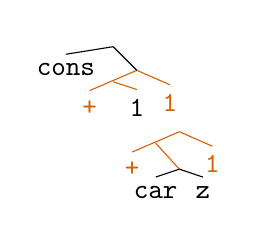
\begin{tikzpicture}[scale=0.6]
    
          \node(l1) at (0,0) {};
  \node[color=pop3](p1) at (-1,-1) {\code{+}};
  \node[color=pop3](n1) at (0.7,-0.9) {\code{1}};
  \node(x1) at (0,-1) {\code{1}};
  \draw[color=pop3] (l1.south) -- (p1.north);
  \draw[color=pop3] (l1.south) -- (n1.north);
  \draw[color=pop3] (-0.5,-0.45) -- (x1.north);

  \node(t) at (-0.5,0.5) {};
  \draw (l1.south) -- (t.south);
  \node(c) at (-1.5,-0.2) {\code{cons}};
  \draw (t.south) -- (c.north);
  
  \begin{scope}[shift={(0.9,-1.3)}]
      \node(l1) at (0,0) {};
  \node[color=pop3](p1) at (-1,-1) {\code{+}};
  \node[color=pop3](n1) at (0.7,-0.9) {\code{1}};
  %\node(x1) at (0,-1) {};
  \draw[color=pop3] (l1.south) -- (p1.north);
  \draw[color=pop3] (l1.south) -- (n1.north);
  \draw[color=pop3] (-0.5,-0.45) -- (0,-1);


  \node(c) at (-0.5,-1.5) {\code{car}};
  \node(z) at (0.5,-1.5) {\code{z}};

  \draw (0,-1) -- (c.north);
  \draw (0,-1) -- (z.north);

%  \node [rotate=90] at (-2.3,-0.7) {\small program};
  
  \end{scope}



\end{tikzpicture}
    };

    \end{tikzpicture}}
  
  \end{minipage}



\end{frame}

\begin{frame}{Explore/Compress/Compile as {\color{red}Amortized} Bayesian Inference}
  
\newcommand{\NeuralNetwork}[1]{    \begin{tikzpicture}[x=2.5cm,y=1.25cm,transform canvas={scale=#1,shift={+(-1,2.5)}}]
      \tikzstyle{neuron}=[circle,fill=blue!50,minimum size=20pt]
      \fill[fill=white] (-0.25,-0.5) rectangle (2.25,-4.5);
      \node[rectangle] at (1,1) {};
      \foreach \name / \y in {1,...,4}
          \node[neuron] (I-\name) at (0,-\y) {};
      \foreach \name / \y in {1,...,3}
          \node[neuron] (H-\name) at (1,-\y-0.5) {};
      \foreach \name / \y in {1,...,4}
          \node[neuron] (O-\name) at (2,-\y) {};
      \foreach \source in {1,...,4}
          \foreach \dest in {1,...,3}
              \draw [-latex] (I-\source) -- (H-\dest);
      \foreach \source in {1,...,3}
          \foreach \dest in {1,...,4}
              \draw [-latex] (H-\source) -- (O-\dest);
    \end{tikzpicture}}

\begin{minipage}[c]{0.4\textwidth}
  \begin{tikzpicture}[scale=1,line width=0.5mm]

  \node[latent,scale=1] at (3.5,3) (dx){DSL};
  \node[latent,scale=1] at ([yshift=-1.5cm,xshift=2cm]dx) (zp){prog};
  \node[obs,scale=1] at ([yshift=-1.45cm]zp) (xp) {task};
  \node[latent,scale=1] at ([xshift=2cm]zp) (zp1){prog};
  \node[obs,scale=1] at ([xshift=2cm]xp) (xp1) {task};
  \draw [->] (zp1.south) -- (xp1.north);
  \draw [->] (dx.south) -- (zp1.north);
  \draw [->,red] (xp1.east) to[out = 30,in = -30] node(nn){} (zp1.east);
  
  \node[latent,scale=1] at ([xshift=-2cm]zp) (zp1){prog};
  \node[obs,scale=1] at ([xshift=-2cm]xp) (xp1) {task};
  \draw [->] (zp1.south) -- (xp1.north);
  \draw [->] (dx.south) -- (zp1.north);
  \draw [->,red] (xp1.east) to[out = 30,in = -30] node(nn){} (zp1.east);


  \draw [->,red] (xp.east) to[out = 30,in = -30] node(nn){} (zp.east);
  \draw [->] (dx.south) -- (zp.north);
  \draw [->] (zp.south) -- (xp.north);

  \draw [->,red] ([xshift=2cm]dx.east) -- ([xshift=3cm]dx.east);
  \node at ([xshift=3.2cm]dx.east]) (uses){is};k
  \node at ([xshift=0.5cm]uses.east) (nnn){\NeuralNetwork{0.17}};
  \draw[thin] ([xshift=1.9cm,yshift=0.4cm]dx.east) rectangle
  ([xshift=0.5cm,yshift=-0.3cm]nnn.south);
  \end{tikzpicture}

  \vspace{0.5cm}

  
\visible<4->{  \begin{tikzpicture}[scale=0.8,line width=0.5mm]
    \node at (0,0) {\underline{\textbf{Compile}: Train {\color{red} recognition model}}};
          \node[align=center] at (-3,-1) (d){DSL};
      %    \node at ([xshift = 3cm]d.east) (p2){program};
      \node at ([xshift=2.5cm,yshift = 0cm]d.east) (p1){program};

      \draw[squiggle,-> ] (d.east) -- node[sloped,above]{\footnotesize  sample} (p1.west);

      \node at ([xshift = 2.5cm]p1.east) (t1){ task};

      \draw [-> ] (p1.east) -- node[above]{\footnotesize  run} (t1.west);

      %% \node(f1) at ([yshift=-0.9cm,xshift=1cm]d.south) {\footnotesize progs. for task$_i$};
      %% \node(t) at ([xshift = 2cm]f1.east) (p11){\footnotesize program$_i$, task$_i$};
      %% \draw [->,squiggle ] (f1.east) -- node[above]{\footnotesize  sample} (p11.west);

%      \draw[dashed,cyan,very thick] ([yshift=0.5cm]p1.west) rectangle  ([yshift=-0.5cm,xshift=0.5cm]p11.east);

      \node(n) at ([yshift=-0.8cm,xshift=1.6cm]p1.south) {
        \NeuralNetwork{0.17}};
      \draw [->,red] (t1.south) to[out = -90,in = 0]  ([xshift=0.4cm]n.east);
      \draw [->,red] ([xshift=-0.4cm]n.west) to[out = -180,in = -70]  ([xshift=-0.25cm,yshift=0.1cm]p1.south); 

    \end{tikzpicture}}
\end{minipage}
\begin{minipage}[c]{0.55\textwidth}
  \visible<2->{  \begin{tikzpicture}[scale=0.8,line width=0.5mm]
    \node at (2,1) {\underline{\textbf{Explore}: Infer programs, fixing DSL and neural net}};
    \node at (0,0) (d){DSL};
    \node at ([yshift = -2cm]d) (t){$\text{Task}$};

    \node at ([xshift = 2cm]t) (nn){
      \begin{tikzpicture}[x=2.5cm,y=1.25cm,transform canvas={scale=0.2,shift={+(-1,2.5)}}]
        \tikzstyle{neuron}=[circle,fill=blue!50,minimum size=20pt]
        \fill[fill=white] (-0.25,-0.5) rectangle (2.25,-4.5);
        \node[rectangle] at (1,1) {};
        \foreach \name / \y in {1,...,4}
            \node[neuron] (I-\name) at (0,-\y) {};
        \foreach \name / \y in {1,...,3}
            \node[neuron] (H-\name) at (1,-\y-0.5) {};
        \foreach \name / \y in {1,...,4}
            \node[neuron] (O-\name) at (2,-\y) {};
        \foreach \source in {1,...,4}
            \foreach \dest in {1,...,3}
                \draw [-latex] (I-\source) -- (H-\dest);
        \foreach \source in {1,...,3}
            \foreach \dest in {1,...,4}
                \draw [-latex] (H-\source) -- (O-\dest);
      \end{tikzpicture}
    };
    \node[align = center, text width = 1cm] at ([yshift = 0.9cm,xshift=-0.5cm]nn.north) {\baselineskip=0pt \small Recog. model\par};
    \draw [red,-{>[scale=0.2]}] (t.east) -- ([xshift = -0.5cm]nn.west);

    \node[draw,rounded corners, inner sep = 10] at ([xshift = 4.2cm,yshift = -1cm]) (s){Search};

    \draw [red,->] ([xshift = 0.5cm]nn.east) -- ([yshift = -0.25cm]s.west);
    \draw [->,rounded corners,] (d.east) -- ([yshift = 2cm]nn.center) -- ([yshift = 0.25cm]s.west);

    \node[align=left] at ([xshift=2cm]s.east) (f) {Programs};
    \draw [->  ] (s.east) -- (f.west);

    \draw [->  ,rounded corners] (t.south) -- ([yshift = -0.5cm]t.south) -- ([yshift = -0.5cm] s.south |- t.south) -- (s.south);
  \end{tikzpicture}}

  \vspace{1cm}
  
\visible<3->{  \begin{tikzpicture}[scale=0.4,line width=0.5mm]


    \node at (0,0) (f1){progs. for task$_1$};
    \node at ([yshift = -1.4cm]f1.south) (f2){progs. for task$_2$};
    \node at ([yshift = -1.4cm,xshift=1.5cm]f2.south) (f3){DSL};

    \node(c)[rectangle, rounded corners, draw, minimum width = 3cm, minimum height = 2.5cm, anchor = north west] at (5.2,1) {};
%    \node[anchor=north] at (c.north) {Compression};
    \node at ([yshift=1cm,xshift=-5cm]c.north) {\underline{\textbf{Compress}: Update DSL, fixing programs}};
    \draw [-> ] (f1.east) -- (c.west|-f1.east);
    \draw [-> ] (f2.east) -- (c.west|-f2.east);
    \draw [-> ] (f3.east) -- (c.west|-f3.east);

    \node[right](d) at ([xshift = 1.6cm,yshift = -0.0cm]c.east) {
      \begin{tikzpicture}[scale=0.6]
        \node[align=center] at (0,0) {DSL+};
\begin{scope}[shift={(0.6,-0.5)}]
  \node[pop3](p1) at (-1,-1) {\code{+}};
  \node[pop3](n1) at (0.6,-0.9) {\code{1}};
  \node[pop3](a) at (0,-1) {\code{ }};
  \draw[pop3] (0,0) -- (p1.north);
  \draw[pop3] (0,0) -- (n1.north);
  \draw[pop3] (-0.3,-0.3) -- (a.north);
  \end{scope}
        \end{tikzpicture}
      };
    \draw [-> ] (c.east) -- (d.west);


    \node at (c.center) {
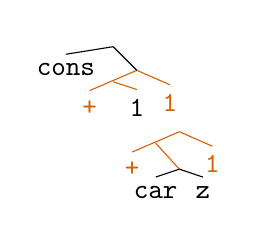
\begin{tikzpicture}[scale=0.6]
    
          \node(l1) at (0,0) {};
  \node[color=pop3](p1) at (-1,-1) {\code{+}};
  \node[color=pop3](n1) at (0.7,-0.9) {\code{1}};
  \node(x1) at (0,-1) {\code{1}};
  \draw[color=pop3] (l1.south) -- (p1.north);
  \draw[color=pop3] (l1.south) -- (n1.north);
  \draw[color=pop3] (-0.5,-0.45) -- (x1.north);

  \node(t) at (-0.5,0.5) {};
  \draw (l1.south) -- (t.south);
  \node(c) at (-1.5,-0.2) {\code{cons}};
  \draw (t.south) -- (c.north);
  
  \begin{scope}[shift={(0.9,-1.3)}]
      \node(l1) at (0,0) {};
  \node[color=pop3](p1) at (-1,-1) {\code{+}};
  \node[color=pop3](n1) at (0.7,-0.9) {\code{1}};
  %\node(x1) at (0,-1) {};
  \draw[color=pop3] (l1.south) -- (p1.north);
  \draw[color=pop3] (l1.south) -- (n1.north);
  \draw[color=pop3] (-0.5,-0.45) -- (0,-1);


  \node(c) at (-0.5,-1.5) {\code{car}};
  \node(z) at (0.5,-1.5) {\code{z}};

  \draw (0,-1) -- (c.north);
  \draw (0,-1) -- (z.north);

%  \node [rotate=90] at (-2.3,-0.7) {\small program};
  
  \end{scope}



\end{tikzpicture}
    };

    \end{tikzpicture}}
  
  \end{minipage}



  \end{frame}


%% \begin{frame}{Compress: Growing the DSL}
%%   \begin{figure}[h!]\tabcolsep=2pt
%% \centering  \begin{minipage}[c]{0.2\textwidth}
%%   \begin{tikzpicture}[scale=0.7]
%%     %% \node[rotate=30] at (-2,0) {\begin{tabular}{c}
%%     %%     \footnotesize Program:\\
%%     %%     \code{($\lambda$ (x) (+ (- x) 1))}
%%     %% \end{tabular}};
%%     %\node at (,0.5) {\code{cons}};
%%     \node [rotate=90] at (-2.3,-0.5) {\small program};
    
%%           \node(l1) at (0,0) {};
%%   \node[color=pop3](p1) at (-1,-1) {\code{+}};
%%   \node[color=pop3](n1) at (0.7,-0.9) {\code{1}};
%%   \node(x1) at (0,-1) {\code{1}};
%%   \draw[color=pop3] (l1.south) -- (p1.north);
%%   \draw[color=pop3] (l1.south) -- (n1.north);
%%   \draw[color=pop3] (-0.5,-0.45) -- (x1.north);

%%   \node(t) at (-0.5,0.5) {};
%%   \draw (l1.south) -- (t.south);
%%   \node(c) at (-1.5,-0.2) {\code{cons}};
%%   \draw (t.south) -- (c.north);
  
%% %    \draw  (l1.south) -- (-0.5,0.5);

%%   %% \node(c) at (-0.5,-1.5) {\code{-}};
%%   %% \node(z) at (0.5,-1.5) {\code{x}};

%%   %% \draw (0,-1) -- (c.north);
%%   %% \draw (0,-1) -- (z.north);
  
%%   \begin{scope}[shift={(0,-2.5)}]
%%       \node(l1) at (0,0) {};
%%   \node[color=pop3](p1) at (-1,-1) {\code{+}};
%%   \node[color=pop3](n1) at (0.7,-0.9) {\code{1}};
%%   %\node(x1) at (0,-1) {};
%%   \draw[color=pop3] (l1.south) -- (p1.north);
%%   \draw[color=pop3] (l1.south) -- (n1.north);
%%   \draw[color=pop3] (-0.5,-0.45) -- (0,-1);


%%   \node(c) at (-0.5,-1.5) {\code{car}};
%%   \node(z) at (0.5,-1.5) {\code{z}};

%%   \draw (0,-1) -- (c.north);
%%   \draw (0,-1) -- (z.north);

%%   \node [rotate=90] at (-2.3,-0.7) {\small program};
  
%%   \end{scope}

%% \begin{scope}[shift={(0,-5)}]
%%   \node[pop3](p1) at (-1,-1) {\code{+}};
%%   \node[pop3](n1) at (0.8,-0.7) {\code{1}};
%%   \node[pop3](a) at (0,-1) {\code{ }};
%%   %\node(x1) at (0,-1) {};
%%   \draw[pop3] (0,0) -- (p1.north);
%%   \draw[pop3] (0,0) -- (n1.north);
%%   \draw[pop3] (-0.55,-0.4) -- (a.north);
%%   \node [rotate=90] at (-2.3,-0.7) {\small fragment};

%%   \end{scope}

%% \end{tikzpicture}
%%   \end{minipage}
%% \hspace{0.1cm}\begin{tabular}{ll}
%%     \toprule
%%     Programs discovered during Explore&Proposed $\lambda$-expression\\\midrule
%%     %% \begin{tabular}{l}
%%     %%   \code{($\lambda$ ($\ell$) (map ($\lambda$ (x) (index x $\ell$))}\\
%%     %%   \phantom{\code{($\lambda$ ($\ell$) (}}\code{(range (- (length $\ell$) 1))))}\\
%%     %%   \code{($\lambda$ ($\ell$) (map ($\lambda$ (x) (index x $\ell$))}\\
%%     %%   \phantom{\code{($\lambda$ ($\ell$) (}}\code{(range (+ 1 1))))}\\
%%     %% \end{tabular}&
%%     %% \begin{tabular}{l}
%%     %%   \code{(map ($\lambda$ (x) (index x $\ell$))}\\
%%     %%   \phantom{\code{(map)}}\code{(range $\alpha$))}\\
%%     %% \end{tabular}\\\midrule
%%     \begin{tabular}{l}
%%       \code{($\lambda$ (s) (map ($\lambda$ (x)}\\
%%       \hspace{0.4cm}\code{ (if (= x '.') '-' x))) s)}\\
%%       \code{($\lambda$ (s) (map ($\lambda$ (x) }\\
%%       \hspace{0.4cm}\code{ (if (= x '-') ',' x))) s)}\\
%%       \end{tabular}&
%%     \begin{tabular}{l}      \code{($\lambda$ (s) (map ($\lambda$ (x)}\\\hspace{0.2cm}\code{   (if (= x $\alpha$) $\beta$ x))) s)}
%%       \end{tabular}
%% \\\bottomrule\\
%% \end{tabular}
%% \caption{\textbf{Left:} syntax trees of two programs sharing common structure,
%% highlighted in {\orange{orange}},
%%   from which we extract a fragment and add it to the DSL (bottom). \textbf{Right:} actual programs,
%%   from which we extract fragments that perform character substitutions.}\label{fragmentExample}
%% \end{figure}

%% \end{frame}

%% \begin{frame}{Compile: Learning to search for programs}
%%   \begin{tikzpicture}[scale=0.85,line width=0.5mm]
%%     \node(x)[draw,align=center] at (0,0) {Task $x$\\e.g., input/outputs};
%%     \node(e)[draw, align=center] at ([xshift=3cm]x.east) {Encoder\\
%%       e.g., RNN or CNN};
%%     \node(m)[draw,align = center] at ([xshift=1.8cm]e.east) {MLP};%\\Output: $(|\mathcal{D}| + 2)\times(|\mathcal{D}| + 1)\times A$};
%%     \node[draw,align = center](s) at ([xshift=3cm]m.east) {Enumerate\\(Explore)};
%%     \node(f)[draw,align = center] at ([xshift=2cm]s.east) {Programs\\solving $x$};

%%     \draw[->] (x.east) -- (e.west);
%%     \draw[->] (e.east) -- (m.west);
%%     \draw[->] (m.east) -- (s.west);
%%     \draw[->] (s.east) -- (f.west);
%%     \draw[->] (x.north) -- ([yshift=15]x.north) -- node[above = 0pt,midway](likelihood){\small likelihood $\probability[\text{task}|\text{prog}]$}([yshift=15,xshift=40]s.north) -- ($(s.east)!0.5!(f.west)$);
%%     \draw[decoration = {brace,mirror,raise = 5pt},decorate,thick]
%%     ([xshift = -5,yshift = -25]e.west) -- node[below = 3pt] {{Recognition model $Q(\text{prog}|\text{task})$}} ([xshift = 180,yshift = -25]e.west);
%%     \draw[decoration = {brace,mirror,raise = 5pt},decorate,thick]
%%     ([xshift = -5,yshift = -25]s.west) -- node[below = 3pt] {{ Search}} ([xshift = 5,yshift = -25]f.east);
%%     %% \draw[decoration = {brace,mirror,raise = 5pt},decorate,thick]
%%     %% ([xshift = -5,yshift = -25]p.west) -- node[below = 3pt] {{\small Params}} ([xshift = 5,yshift = -25]p.east);
%%     \node at ([yshift=0.5cm]likelihood.north) {\textbf{\underline{Inference at test time (\underline{Explore Step})}}};
%%   \end{tikzpicture}

%%   \vspace{0.5cm}
  
%%   \centering\emph{\textbf{Minimize Loss}}: $\text{KL}(\text{P}\left[\text{prog}|\text{DSL},\text{task} \right] || Q(\text{prog}|\text{task}))$

%%   \vspace{0.5cm}
%%   \begin{tikzpicture}[scale=1,line width=0.5mm]
%% \visible<2->{    \node at (0,0) (f1){progs. for task$_1$};
%%     \node at ([yshift = -0.6cm]f1.south) (f2){progs. for task$_2$};
%%     %    \node at ([yshift = -1cm]f2.south) (f3){progs. for task$_3$};

%%     \node at ([xshift = 2cm]f1.east) (p1){program$_1$, task$_1$};
%%     \node at ([xshift = 2cm]f2.east) (p2){program$_2$, task$_2$};
%%     %    \node at ([xshift = 2cm]f3.east) (p3){program$_3$, task$_3$};


%%     \draw [->,squiggle ] (f1.east) -- node[above]{\small sample} (p1.west);
%%     \draw [->,squiggle ] (f2.east) -- node[above]{\small sample} (p2.west);
%%     %    \draw [->,squiggle ] (f3.east) -- node[above]{\small sample} (p3.west);
    

%%     \node at ([yshift = 0.5cm,xshift=-1.3cm]p1.north) {\textsc{\textbf{\underline{Training on real data}}}};
%%     }
%%     %% \end{tikzpicture}%
%%     %%   \begin{tikzpicture}[scale=3,line width=1.5mm]
%%     \begin{scope}[shift = {(6cm,-0.5cm)}]

%% \visible<3>{      \node[align=center] at (0,0) (d){DSL};
%%       %    \node at ([xshift = 3cm]d.east) (p2){program};
%%       \node at ([xshift=2cm,yshift = 0.5cm]d.east) (p1){program};
%%       \node at ([xshift=2cm,yshift = -0.5cm]d.east) (p3){program};

%%       \draw[squiggle,-> ] (d.east) -- node[sloped,above]{\small sample} (p1.west);
%%       \draw[squiggle,-> ] (d.east) -- node[sloped,below]{\small sample} (p3.west);

%%       \node at ([xshift = 2cm]p1.east) (t1){task};
%%       \node at ([xshift = 2cm]p3.east) (t3){task};
%%       \draw [-> ] (p1.east) -- node[above]{\small execute} (t1.west);
%%       \draw [-> ] (p3.east) -- node[above]{\small execute} (t3.west);

%%       \node at ([yshift = 0.5cm]p1.north) {\textsc{\textbf{\underline{Training on DSL samples}}}};
%% }    \end{scope}
%%   \end{tikzpicture}
%% \end{frame}

\begin{frame}{Domain: List processing}
      Starts with: \code{foldr}, \code{unfold}, \code{if}, \code{map}, \code{length},
\code{index}, \code{=}, \code{+}, \code{-}, \code{0}, \code{1}, \code{cons},
\code{car}, \code{cdr}, \code{nil}, \code{is-nil},  \code{mod}, \code{*}, \code{>}, \code{is-square}, \code{is-prime}.
\\236 human-interpretable list processing tasks.
\\Discovers 38 new DSL primitives, including \code{filter}

\vspace{0.25cm}

\centering \begin{minipage}[c]{0.6\textwidth}
  \begin{tabular}{lll}
    \toprule
    Name & Input & Output \\\midrule
    repeat-2 & [7\, 0] & [7\, 0\, 7\, 0] \\
    drop-3 & [0\, 3\, 8\, 6\, 4] & [6\, 4] \\
    rotate-2 & [8\, 14\, 1\, 9] & [1\, 9\, 8\, 14] \\
    count-head-in-tail & [1\, 2\, 1\, 1\, 3] & 2 \\
    keep-mod-5 & [5\, 9\, 14\, 6\, 3\, 0] & [5\, 0] \\
    product & [7\, 1\, 6\, 2] & 84 \\
    \bottomrule
  \end{tabular}
\end{minipage}%
%% \begin{minipage}[c]{0.3\textwidth}
%%   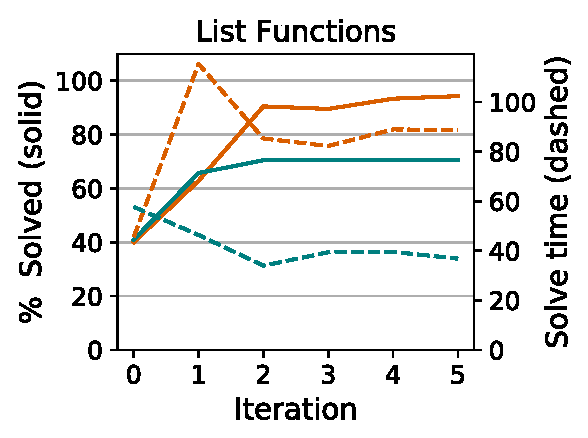
\includegraphics[width = \textwidth]{figures/listLearningCurve_color.eps}
%% {   \color{orange}orange: } full system. {\color{teal}teal: } no neural recognition model
%% \end{minipage}

\vspace{0.25cm}

\centering \textbf{With functional programming ``problem set'' + 93 hours on 64 CPUs, rediscovers:}\\
\textbf{\code{map}, \code{foldr}, \code{unfold}, \code{range}, \code{length}, \code{index}, \code{zip}}, +some arithmetic routines


  \end{frame}

\begin{frame}{Domain: Text Editing}
  In the style of FlashFill (Gulwani 2012). Starts with: \code{foldr}, \code{unfold}, \code{if}, \code{map}, \code{length},
\code{index}, \code{=}, \code{+}, \code{-}, \code{0}, \code{1}, \code{cons},
\code{car}, \code{cdr}, \code{nil}, \code{is-nil}
, plus string \& character constants.\\

\begin{minipage}[c]{0.4\textwidth}
  \begin{tabular}{ll}
    \toprule
    Input&Output\\\midrule
    +106 769-438&106.769.438\\
    +83 973-831&83.973.831
    \\\midrule
          Temple Anna H&TAH\\
      Lara Gregori&LG
    \\\bottomrule 
    \end{tabular}
  %% \begin{figure}
  %% 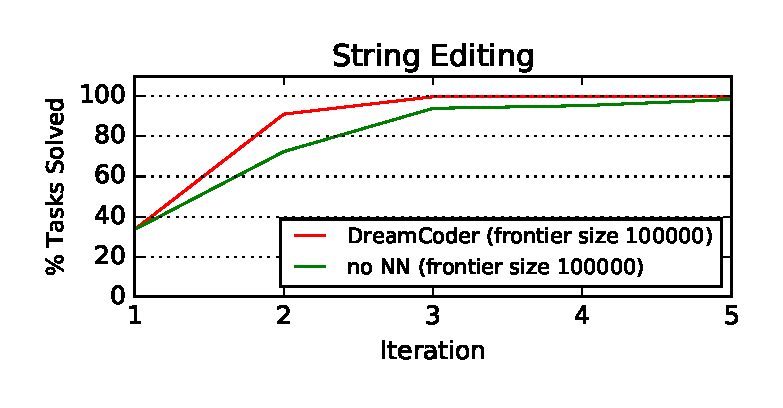
\includegraphics[width = 0.8\textwidth]{figures/textLearningCurve.eps}
  %%   \end{figure}
  \end{minipage}
\begin{minipage}[c]{0.5\textwidth}
      \begin{figure}        
        \includegraphics[width = \textwidth]{figures/textPrimitives.png}\vspace{-0.8cm}
      \caption{11 learned DSL primitives over 3 successive iterations (3 columns). Learned primitives call each other (arrows).}
      \end{figure}  
  \end{minipage}
\end{frame}

\begin{frame}{Domain: Symbolic regression from visual input}
  Starts with: \code{plus}, \code{times}, \code{divide}, \code{real-number}. Autograds through program
  \\  Bayesian likelihood $\probability[\text{data}|\text{prog}]$ favors fewer continuous parameters

  \centering
  %% \begin{minipage}[c]{0.4\textwidth}
  %% \begin{figure}
  %%   \newcommand{\functionSize}{1.5cm}\centering
  %% 
\includegraphics[width = \functionSize]{figures/functions/6.png}
  %% 
\includegraphics[width = \functionSize]{figures/functions/48.png}
  %% 
\includegraphics[width = \functionSize]{figures/functions/102.png}
  %% 
\includegraphics[width = \functionSize]{figures/functions/116.png}\\
  %% \vspace{0.0pt}
\includegraphics[width = \functionSize]{figures/functions/181.png}
  %% 
\includegraphics[width = \functionSize]{figures/functions/160.png}
  %% 
\includegraphics[width = \functionSize]{figures/functions/149.png}
  %%   
\includegraphics[width = \functionSize]{figures/functions/187.png}
  %% \caption{Recognition model input. DSL learns subroutines for polynomials/rational functions (top/bottom) while the recognition  model jointly learns to look at a graph of the function (above) and predict which of those subroutines best explains the observation.}\label{functions}\vspace{-0.5cm}
  %%   \end{figure}    
  %% \end{minipage}
  %
\centering

\vspace{1cm}\begin{tabular}{cc}
    \toprule
\normalsize \pop{Programs} \& Tasks&\normalsize \popp{DSL}\\\midrule 
\small    \begin{tabular}{cc}
      
\includegraphics[width = 3em]{figures/functions/4.png}&
      
\includegraphics[width = 3em]{figures/functions/146}\\
      \pop{\code{$f($x$) = $($f_1$ x)}}&    \pop{\code{$f($x$) = $($f_5$ x)}}\\
%      ~\\
      
\includegraphics[width = 3em]{figures/functions/112.png}&
        
\includegraphics[width = 3em]{figures/functions/92.png}
      \\
      \pop{\code{$f($x$) = $($f_4$ x)}}&    \pop{\code{$f($x$) = $($f_3$ x)}}\\

    \end{tabular}
&    \small
    \begin{tabular}{l}
    \popp{$f_0($\code{x}$)\,=\,$\code{(+ x real)}}\\
    \popp{$f_1($\code{x}$)\,=\,$\code{($f_0$ (* real x))} }\\
    \popp{$f_2($\code{x}$)\,=\,$\code{($f_1$ (* x (}$f_0$\code{ x)))}}\\
    \popp{$f_3($\code{x}$)\,=\,$\code{($f_0$ (* x (}$f_2$\code{ x)))}}\\
    \popp{$f_4($\code{x}$)\,=\,$\code{($f_0$ (* x (}$f_3$\code{ x)))}}\\
    \hspace{\helpSize}\emph{($f_4$: 4th order polynomial)}\\
    \popp{$f_5($\code{x}$)\,=\,$\code{(/ real ($f_0$ x))}}\\
    \hspace{\helpSize}\emph{($f_5$: rational function)}\\

  \end{tabular}
  \\\bottomrule\\
\end{tabular}
  \end{frame}

\begin{frame}{New domain: Generative  graphics  programs (Turtle/LOGO)}
  \begin{tabular}{cc|c}
    Training tasks& DSL samples before learning&DSL samples after learning\\
              \raisebox{-.5\height}{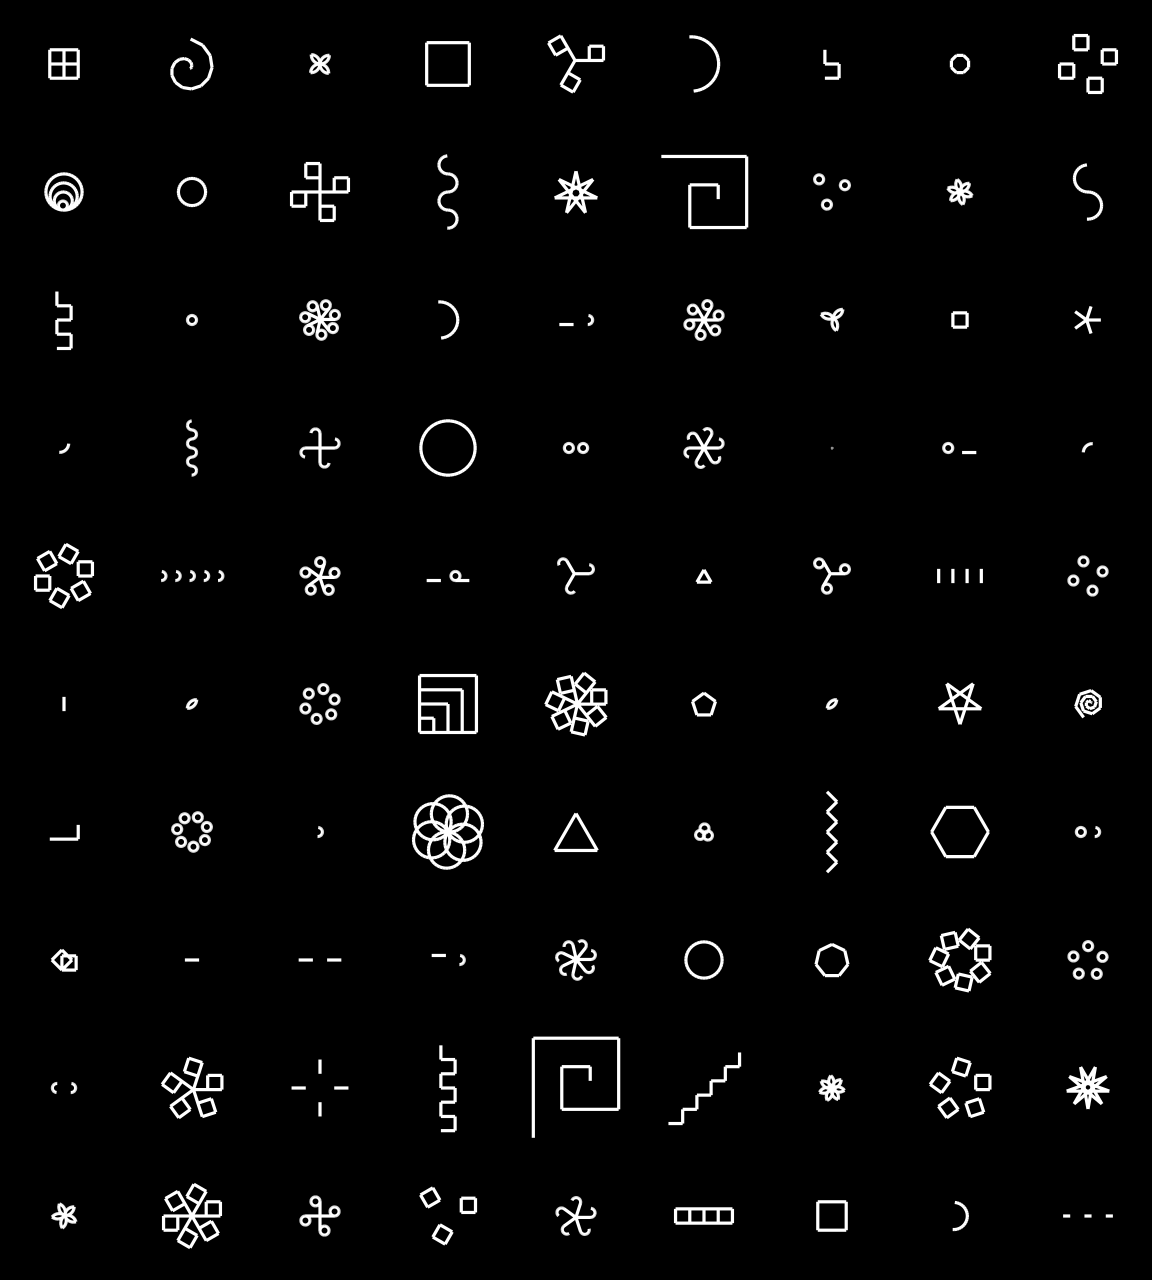
\includegraphics[width = 0.2\textwidth]{figures/logo90.png}$\quad\quad$ }&
      \raisebox{-.5\height}{\includegraphics[width = 0.3\textwidth]{figures/initialDreams/montage.png}}&
  \raisebox{-.5\height}{\includegraphics[width = 0.3\textwidth]{figures/finalDreams/montage.png}}
  \end{tabular}

  \vspace{0.3cm}

  \pause
  
  Learned DSL contains parametric drawing routines:
      \begin{tabular}{rlrl}
      Semicircle:& \raisebox{-.5\height}{\includegraphics[width = 0.3\textwidth]{figures/logo_primitives/logo_primitive_24.png}}&
      Spiral:&\raisebox{-.5\height}{\includegraphics[width = 0.3\textwidth]{figures/logo_primitives/logo_primitive_25.png}}\\
      Greek Spiral:&\raisebox{-.5\height}{
\includegraphics[width = 0.3\textwidth]{figures/logo_primitives/logo_primitive_10.png}}&
      S-Curves:&\raisebox{-.5\height}{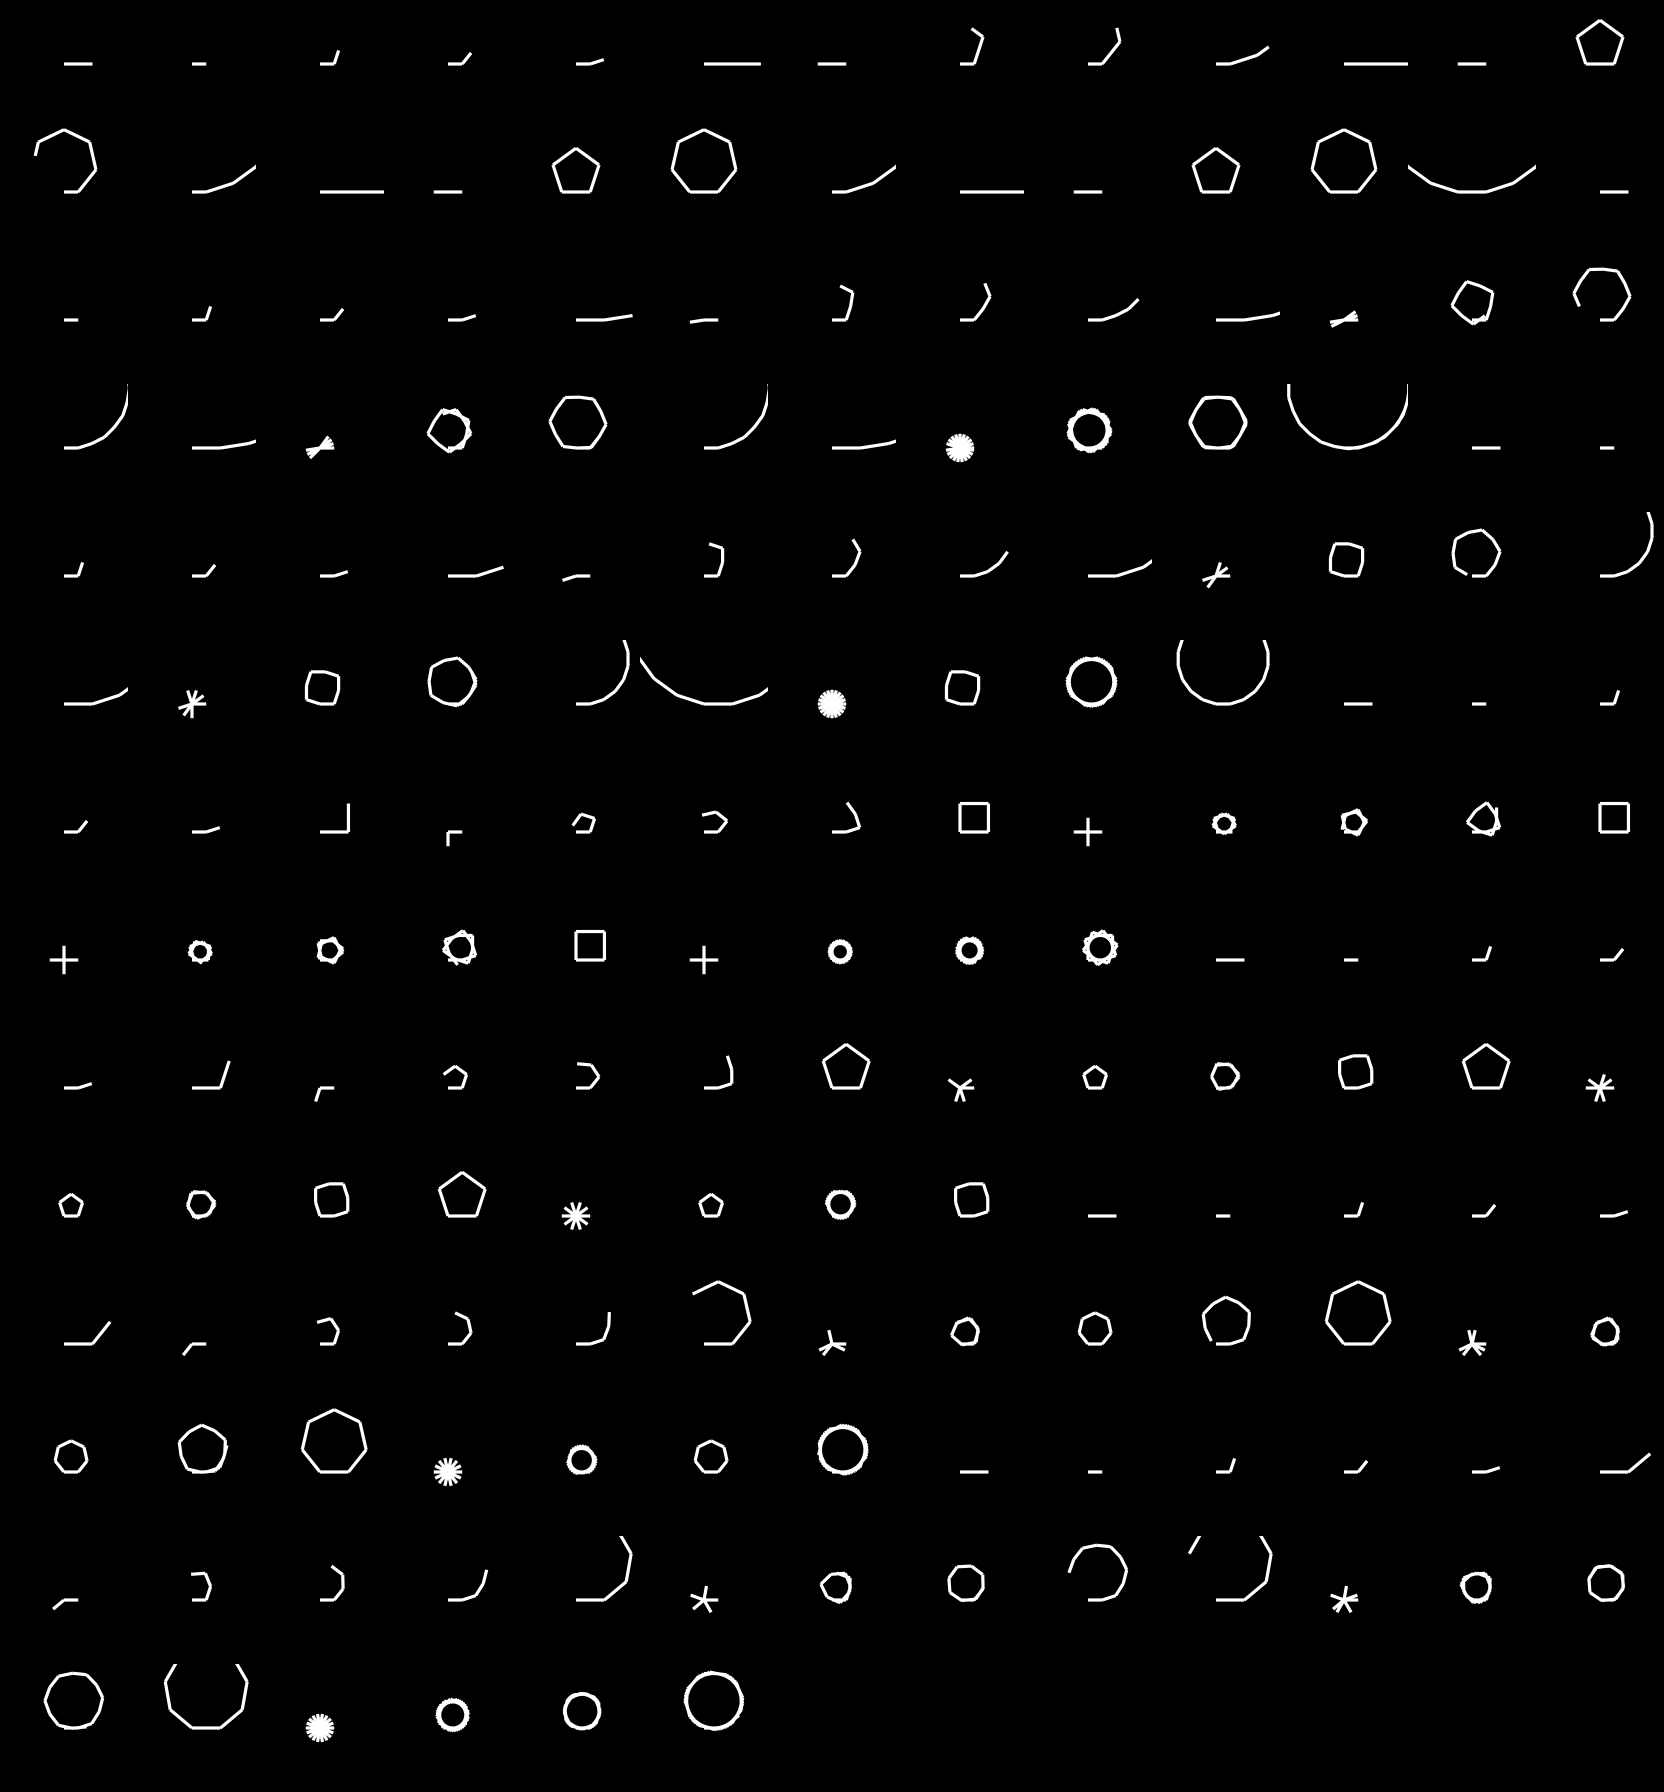
\includegraphics[width = 0.3\textwidth]{figures/logo_primitives/logo_primitive_11.png}}        \\
        Polygons \& Stars:
        &\raisebox{-.5\height}{
\includegraphics[width = 0.3\textwidth]{figures/logo_primitives/logo_primitive_12.png}}&
                Circles:
&\raisebox{-.5\height}{\includegraphics[width = 0.3\textwidth]{figures/logo_primitives/logo_primitive_23.png}}
    \end{tabular}
  
  

  \end{frame}


\end{document}
